%%%%%%
%%
%%  Don't reorder the reviewer points; that'll mess up the automatic referencing!
%%
%%%%%

\begin{minipage}[b]{2.5in}
  Resubmission Cover Letter \\
  {\it Genetics}
\end{minipage}
\hfill
\begin{minipage}[b]{2.5in}
    Han Li \\
    \emph{and} Peter Ralph \\
  \today
\end{minipage}
 
\vskip 2em
 
\noindent
{\bf To the Editor(s) -- }
 
\vskip 1em

We are pleased to finally submit a revised version of our manuscript, 
``Local PCA shows how the effect of population structure differs along the genome'',
previously submitted with ID GENETICS/2016/197517.
As you will see, at the reviewers' requests 
we have put substantial effort into additional validation of the method,
including simple simulations to back up some of our mathematical claims about the method
(e.g., about PC switching),
and individual-based simulations with large numbers of loci under weak selection
on realistically-sized chromosomes.
The latter simulations, 
which verify that our method can detect the action of linked selection,
were made possible with tools only recently developed (in part by us).
Our additional tests are described in Section \ref{ss:testing_methods}.

In adding simulation results and the additional verifications requested by the reviewers,
we have endeavored not to expand the manuscript (or the supplementary figures) too much.

Besides these additional verifications,
we have tried to shift the focus away from background selection specifically
to more general linked selection.
We think it likely that background selection is a contributing factor,
but that the relative contributions of different sorts of selection
on genomic landscapes of diversity, divergence, and relatedness
are almost completely unknown, and constitute a major open question in the field.
We hope this addresses Reviewer 1's skepticism regarding background selection.

In addition to the main document, with line numbers and hyperlinked references
from the responses to reviews,
we have also uploaded a version highlighting the changes between this version
and the submitted one (note that the submission system doesn't provide an appropriate category
for this file upload, so it is also marked ``Response to Reviewers'').

We hope you find the manuscript to be improved as much as we do.

\noindent \hspace{4em}
\begin{minipage}{3in}
\noindent
{\bf Sincerely,}

\vskip 2em

{\bf 
Han Li and
Peter Ralph
}\\
\end{minipage}

\vskip 4em

\pagebreak
\setcounter{page}{1}

%%%%%%%%%%%%%%
\reviewersection{AE}

\begin{quote}
    Adding simulations to strengthen key claims will be necessary, particularly
    addressing the impacts of mutation rate and recombination rate variation
    with more depth, the concern regarding PC switching (Reviewer 1), and the
    concern regarding the impacts of variation in missingness by sub-population
    (Reviewer 2).
\end{quote}

Thanks for the positive feedback and the useful suggestions.
We agree that more extensive exploration 
using simulations would help bolster understanding of the method,
and have now done so.
See below for more detailed responses.


%%%%%%%%%%%%%%
\reviewersection{1}

\begin{quote}
    The paper is generally well written and clear; it addresses an important
    problem, and clearly makes some progress on it. However, it suffers from having
    no grounding in either theory or empirical demonstration that it really can find
    the structures that are claimed. I find the arguments that it finds inversions
    compelling, though not watertight, and I am not yet convinced that it is finding
    ubiquitous background selection.  To make this claim, significant extra work is
    required.

    In short, the approach is interesting but not sufficiently explored to produce
    compelling evidence for the implications that are claimed.  Putting a large
    amount of effort into simulations may alleviate these concerns somewhat.
\end{quote}

We have backed off somewhat on our previous speculation that the observed patterns
are due to background selection,
and have also put a large amount of effort into simulations (discussed below).
We hope these alleviate your concerns.

\begin{quote}
    Specific points: What does this method find? I'm concerned about:
    (a) variation in the recombination rate
    and (b) variation in the mutation rate, creating spurious structure.

    The first possibility is that massively varying information quantity
    within windows could lead to a small number of such windows having their
    orientation reversed: that is, PC1 becomes PC2 and vice versa. (Or PC2 and PC3
    could switch). This would lead to such windows having unusual properties and
    hence appearing as evidence of an inversion.

    I do agree with the authors that significant outliers would be found at
    inversions. However, even if the PC switching does not occur, or the model could
    handle it, the evidence for selection is weaker.  If the two types of variation
    described above exist, with no selection, I would still expect a ``continuous
    triangle'' of results (as seen left of Fig 2, top left of Fig 6) with extrema
    described by windows with the most information, and points placed at different
    extremum having low recombination rate (because by chance, these will get an
    approximately fixed local tree, corresponding on average to the genome-wide
    population structure).

    Addressing this is likely quite hard, though the authors may be able to think of
    something that separates these effects from selection.
\end{quote}

Specific points are addressed below.
Briefly, switching of PC 1 and 2 cannot mislead the method
because we measure distances in a way that does not depend on PC ordering.
It is possible that switching of PC 2 and 3 could mislead if we are using only $k=2$ of the PCs;
however, we see the same patterns when using more PCs, so we know this is not happening.

As for inversions: we aren't claiming that every strong localized signal discovered by this method
is an inversion (and we've tried to make sure the paper doesn't imply that!),
but think we have good evidence for the taxa we study.
We hope the reviewer agrees that we find the large inversions of \emph{Drosophila},
where (a) PCA structure coincides with known inversion breakpoints, 
and (b) the local PCA plots separate samples carrying the two inversion orientations.
Nearly all of the inversion-like signals we find in human are likewise located at the positions 
of known polymorphic inversions; 
however, we agree that the evidence for remaining inversion is \emph{not} watertight,
because, as the reviwer points out (and we do as well),
we cannot distinguish them from long regions of low recombination.
The fact that nearly all of the strong, localized signals coincide with known polymorphic inversions
induces us to emphasize inversions.
We now more clearly emphasize this caveat in the Discussion \llname{ll:inversion_caveat}.

\begin{point}{}
    \ldots (a) variation in the recombination rate and 
    (b) variation in the mutation rate \ldots creating spurious structure.
\end{point}

\reply{
    We have now added simulation tests showing that large-scale variation in recombination rate
    does not create spurious structure \llname{ll:test_recomb_rate};
    except in the presence of long regions of low recombination,
    which we point is is as expected \llname{ll:hotspot_recomb}.
    We also check for the effect of this in the real data:
    since we only look at SNPs,
    a 1Kb window with mutation rate $\mu$ and recombination rate $\rho$
    is equivalent to a 10Kb window with mutation rate $\mu/10$ and recombination rate $\rho/10$,
    and the ratio $\mu/\rho$ determines the ``signal-to-noise'' ratio.
    Therefore, we can check for effects due to recombination
    and mutation rate variation 
    by comparing results with windows of different types --
    windows of equal length in bp, or in SNPs, have different lengths in cM.
    These different choices show nearly identical patterns in all cases we have examined,
    as is summarized in Table \ref{tab:window_sizes},
    making it unlikely that recombination or mutation rate variation could be driving the results.
}

\begin{point}{PC switching}
\ldots could lead to a small number of such windows having their
orientation reversed: that is, PC1 becomes PC2 and vice versa. (Or PC2 and PC3
could switch).
\end{point}

\reply{
    This is a natural concern.
    However, the only point at which we compare PCs in a way that could be sensitive to ordering
    is in determining the window size -- we compute the distance between windows
    in a way that is invariant under ordering.
    We have made this more clear by moving the note about flipping signs of PCs
    to the appendix on window choice \llname{ll:moved_pc_note}
    and added more explicit notes about this to \llname{ll:another_pc_point} and \revref.
    Furthermore, one of our simulation tests
    is explicitly designed to test for this effect. \llname{ll:pc_switching_test}
}

\begin{point}{p6}
``here, we use k=2...''  - you have to show that $k>2$ is the same.
\end{point}

\reply{
    We have added a table including correlations between MDS values between $k=2$ and $k=5$
    for the Medicago data (Table \ref{tab:param_cors}),
    and a representative figure (for the Drosophila data, $k=5$),
    see Figure \ref{sfig:dmel_k5}, \revref and \llname{rr:rev1:4}.
}

\begin{point}{p15}
``We also found nearly identical results when choosing shorter windows of 1,000 SNPs'' - again, show this.
\end{point}

\reply{
    The same table includes correlations between MDS values for different window lengths 
    (Table \ref{tab:param_cors}). \revref
}

\begin{point}{p15}
 ``or choosing windows of equal length in base pairs rather than SNPs'' - once again.
\end{point}

\reply{
    Again, we address this in Table \ref{tab:param_cors}. \revref
}

\begin{point}{}
Using 2 PCs is common practice: only if this is the end of an analysis and the
PCA was done for visualization. Here you are using it for something so should
keep all the relevant PCs.
\end{point}

\reply{
    This is a good point; the question is which the ``relevant'' PCs are.
    \citet{novembre2008interpreting} showed that under isolation by distance,
    the top two PCs should reflect the two-dimensional nature of the range,
    and higher PCs are generally much less interpretable;
    we used $k=2$ with this in mind.
    We have changed this sentence \revref.
}

\begin{point}{}
I'm surprised that PCAdmix isn't referenced. It is using a very similar
method, albeit with different goals. In particular, the approach of placing all
points into a single, genome-wide PC space solves many of the problems that this
approach has (though I agree there may be benefits to the approach described here)
\end{point}

\reply{
    Good point: we now reference this work and discuss it's similarity. \revref
}

%%%%%%%%%%%%%%
\reviewersection{2}

\begin{quote}
    This is an interesting and well written paper. It was a pleasant read. I have three main general
    comments:
\end{quote}

Thanks! We're glad you enjoyed it.

\begin{point}{Related work:} 
The authors provide an introduction of the main concepts, as well as some
intuition of what the method is doing and how, but I found comparison to previous approaches
to be somewhat missing. To some extent, this is due to the fact that the main goal of their
analysis is somewhat vaguely ``finding heterogeneity'', which leads to the applications of
detecting chromosomal inversions and evidence for background selection. It would help to
have a well defined set of hypotheses, test the method's accuracy using simulation (see next
comment), and compare to previous efforts in similar domains.
\end{point}

\reply{
    First: we think that ``finding heterogeneity'' is in fact a well-defined goal,
    although it was not that well-defined in the paper;
    we have hopefully improved on this in the Introduction \revref.
    Expanding a bit more:
    We agree that methods that seek to test well-defined hypotheses
    are extremely useful and powerful.
    We feel that methods for visualization and exploration are also useful --
    a primary example here being PCA (as used for visualization).
    If PCA is useful -- or more generally, dimension reduction --
    then it should be important to also know how much the thing that PCA is summarizing
    varies along the genome,
    in the same way that knowing the mean of some quantity in a population 
    is only of limited usefulness
    without also knowing the corresponding population variance.
}

\begin{point}{Validation:}
In several occasions, the authors seem to introduce a potential problem in their
approach, and provide a solution to it. This is generally rather intuitive, but it would really help
to have simulations of some sort to show that the issue arises and leads to a problem, and that
their approach does address the specific problem.
\end{point}

\reply{
    We have added a number of simulations testing various aspects of the method,
    and have tried to incorporate the results in the paper without cluttering it up
    with the results of sanity checks.
    See sections \ref{ss:testing_methods} and \ref{ss:validation};
    in particular the Gaussian simulations described in appendix \ref{apx:gaussian_sims}.
}


\begin{point}{}
The use of weighted PCA to cope with unbalanced sample size could be better demonstrated.
Although the current explanation makes intuitive sense, this approach does not seem to be
used in previous work. The authors could design a simulation that supports their approach.
\end{point}

\reply{
    We felt that weighted PCA was a nice but unnecessary complication to this work,
    so have removed it entirely.
}


\begin{point}{}
It is conceivable that some subpopulations will have more missingness in some windows. That
may skew the resulting PCs by selecting different sample sizes for the different windows (as
discussed in Appendix B). This could distort the PCs, so that variation reflects underlying
variation in missingness. Would be good to discuss this potential issue and provide simulations.
\end{point}

\reply{
    We have tested the method against a large quantity of missing data
    in which the amount of missingness does not vary by population \llname{ll:test_missing}.
    However, missingness that is structured by population could absolutely cause variation in PCs.
    This could happen, for instance, with RAD data wherein allelic dropout is driven by
    population-specific polymorphism in the restriction site.
    The same problem to a lesser degree would be caused by mapping bias,
    and in fact we see windows around the breakpoints of the polymorphic inversions
    of the DPGP data having higher rates of missingness.
    We definitely would like our method to be insensitive to missing data,
    but if missingness is in fact correlated with the signal we are looking for 
    (changes in patterns of relatedness, as it is in these cases),
    correlation of MDS scores with amount of missingness is not in fact a problem.
    As we don't think this point is particularly helpful to the reader, 
    we have provided a plot of missingness against MDS score (Figure \ref{sfig:dpgp_missingness})
    and mentioned it in the text \revref,
    but have not added a lengthy discussion.
}

\begin{point}{Appendix A:}
when using jackknife to estimate variance, each window is being divided in 10
``independent'' resampling units. Due to LD, these 10 blocks are likely correlated, which would
bias the estimates of variance. This is probably not a problem because both signal and noise
could be equally biased, but the authors may want to consider this potential issue. I wonder if
the correlation with recombination rate may be partially explained by this.
\end{point}

\reply{
    That's true, but we are unaware of a better option,
    and since the jackknife is only used to pick an appropriate window size,
    it does not seem crucial.  {\revref}
    Since results are the same across different window sizes,
    we don't think this can explain a correlation with recombination rate.
}

\begin{point}{}
Is it possible to explain the results of Figure 6 just considering neutral variation in local
ancestry due to recent admixture? This may explain why ancestry seems to explain a fair
amount of variance in the lower plots of Fig 6. Local PCA has been previously used by others to
detect local ancestry blocks, e.g. see the PCAdmix approach by Brisbin et al. The authors
discuss the possibility that admixture is driving the differentiation, but do not test whether their
observations agree with neutrality.
\end{point}

\reply{
    This is a good point, but any \emph{neutral} variation in local ancestry
    is not expected to vary systematically along the chromosome,
    as we now discuss more explicitly \llname{ll:not_neutral}.
    It well could be that the patterns we see are due to selection acting differentially
    on introgressed segments,
    a scenario that would fall under ``linked selection''.
    We discuss this in the Discussion \revref.
    We also now cite and discuss the differences to PCAdmix \revreffull{1}{7}.
}

\begin{point}{}
``to remove the effect of artifacts such as mutation rate variation, we also rescale each
approximate covariance matrix to be of similar size (precisely, so that the underlying data
matrix has trace norm equal to one''. This potential issue is a bit unclear to me, since I would
expect that scaling the volume of local trees would not result in changed distances in PC
space. Perhaps the authors could show via simulations that this creates a problem, and that the
normalization addresses it.
\end{point}

\reply{
    We agree that demonstrating this issue would be nice in principle,
    but think that for this audience would be getting too far down in the weeds.
    (Besides, we aim to provide a good method, not to prove that the method
    is better than all other possible methods.)
    For the reviewer's sake, here is some more about our rationale.
    Suppose that the covariance matrix is the same along the whole genome,
    except that it is multiplied by an overall constant that varies.
    Since PCs are scaled to have norm 1, this overall scaling will indeed not affect the PCs,
    but we don't compare the PCs directly -- we compare the low-dimensional approximations
    to the covariance matrix, and the scaling we propose would remove the effect
    of this overall constant.
    It is not clear that variation in mutation rate would act like an overall multiple
    of the covariance matrix, but
    since we're interested in patterns rather than magnitudes of relatedness,
    it seems a wise thing to remove.
}

\begin{point}{Figure 7:}
    Are MDS coordinates correlated with recombination rates in this case?
\end{point}

\reply{
    We made a stab at checking this,
    and obtained the best version to date of the Medicago recombination map
    from Tim Paape and Peter Tiffin.
    There are two versions: a very coarse physical map, and a fine-scale map estimated using LDhat.
    However, both are on version 3.0 of the assembly,
    while all other coordinates (sequencing data; gene annotations) are in version 4.0.
    Furthermore, as Peter Tiffin told us,
    ``apparently there are no files that translate Mt3.0 to Mt4.0 locations (yes, seems a bit silly)."
    There is a liftOver chain file for translating 3.5 to 4.0, and
    ``the differences in the Mt3.0 and Mt3.5 assemblies are, however, apparently relatively minor''.
    On this basis, we produced the desired figure assuming that Mt3.0 coordinates
    are the same as Mt3.5 coordinates, included to satisfy the reviewers' curiosity: \\
    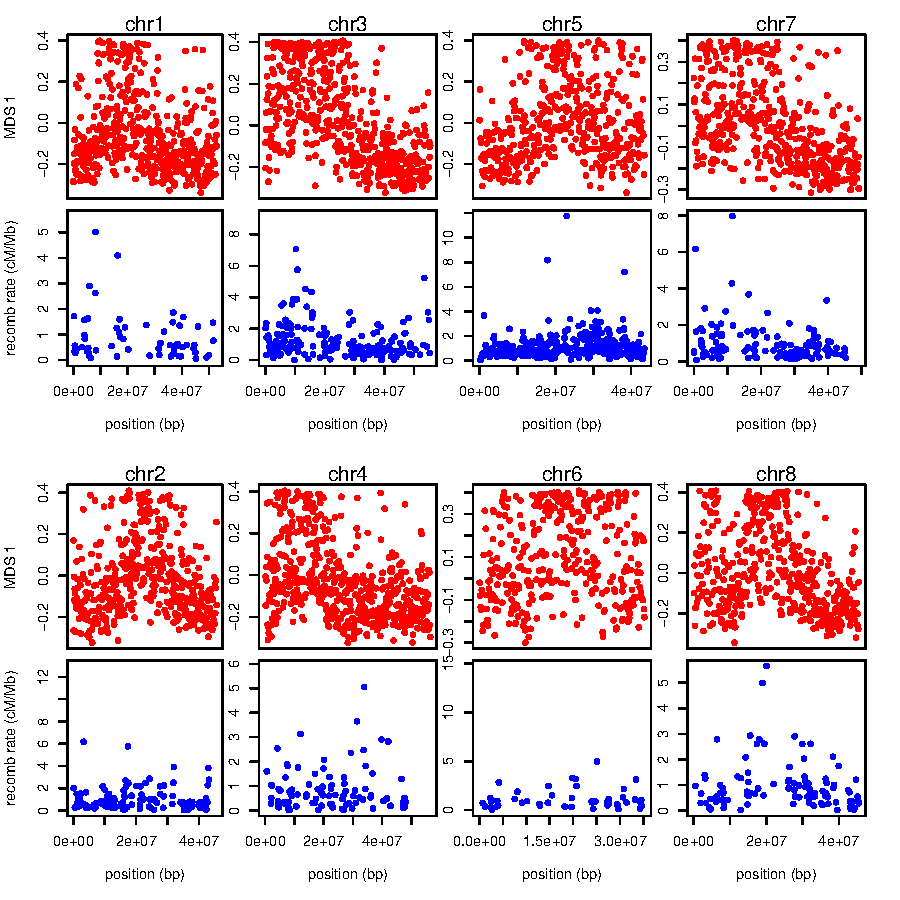
\includegraphics{../medicago/recomb_rates/recomb_and_mds} \\
    However, given uncertainties in this mapping, the relatively poor match of window sizes,
    the large number of unmappable windows, and the nature of the recombination data
    (produced with LDhat, not with actual observations of recombinations),
    we decided not to include this (but have provided a note, \revref).
}

\begin{point}{Application:}
Is what the authors seem to be proposing not already accounted for by linear
mixed model association approaches? If not, this should be clarified. Either way, this paragraph
could be dropped.
\end{point}

\reply{
    It is not accounted for; we've added some more explanation to this section
    (which we think should stay in). \revref
}

\begin{point}{Introduction:}
 ``it is not necessarily clear what aspects of demography should be included in the
concept.'' I find it a bit weird to describe selection as an ``aspect of demography''. Although it
could be seen as such within a coalescent framework, that seems to be just a useful
representation. The authors may consider rewording.
\end{point}

\reply{
    Good point, but we think that the sense of unease is perhaps desirable here:
    certainly differential survival is an aspect of demography;
    but as the rest of the paragraph goes on to discuss,
    this quickly spills over into selection, which probably should not be included.
    We've opted to keep this. \revref
}

\begin{point}{}
Paragraph starting in ``Since the definition...''. The notation is a bit unclear. Please check that it
is clear which PC the text refers to.
\end{point}

\reply{
    We've rewritten this section;
    hopefully it is clearer. \revref
}

\begin{point}{}
Would the authors be able to provide a sense for the directionality of effects in Figure 4? It
would be interesting if the authors tried to further characterize regions that are similar due to
higher recombination rates. E.g.\ is there more/less density of polymorphisms in these regions?
\end{point}

\reply{
    We agree, that further investigation into these patterns and their correlates
    would be very interesting and fruitful;
    however, we think it's outside of the scope of this paper.
}

\begin{point}{Page 13:}
typo: ``figures 6 and 6''.
\end{point}

\reply{Fixed. \revref}

\begin{point}{}
Typo in abstract, line 6 ``, We show'' $\rightarrow$ ``. We show''.
\end{point}

\reply{Fixed.}

\begin{point}{}
Typo: end of introduction ``an visualization''. The whole sentence is a bit weird. The authors just
stated focus is on clustering, not on looking for outliers, but what does it mean that ``we allow
ourselves to be surprised by unexpected signals in the data''?
\end{point}

\reply{
    We have removed this sentence.
}

\begin{point}{}
``There has been substantial debate over the relative impacts of different forms of selection.''
Citation needed.
\end{point}

\reply{
    We have added some relevant recent citations,
    but apologize for not being aware of the appropriate recent review to refer to.
    \revref
}

\begin{point}{}
``Results using larger numbers of PCs were nearly identical''. It would be interesting to have a
supplementary table.
\end{point}

\reply{
    We have included a table of correlations (Table \ref{tab:param_cors}),
    as well as the plots for Drosophila data using $k=5$
    (Figure \ref{sfig:dmel_k5}),
    and hope that readers will take our word on this point more generally.
}

\begin{point}{}
Table 1 legend seems a bit redundant. Columns are self-explanatory.
\end{point}

\reply{
    Good point; we've cut this down.
}

\begin{point}{}
It would help to have numbered lines and references.
\end{point}

\reply{
    Now provided.
}
